\documentclass[12pt]{article}
\usepackage[margin=4cm]{geometry}
\usepackage{algpseudocode}
\usepackage{algorithm}
\usepackage[utf8]{inputenc}
\usepackage{tikz} 
\usepackage{multicol}
\usepackage{graphicx}
\newcommand\floor[1]{\lfloor#1\rfloor}
\usepackage{amsmath,amsthm,amssymb}
\usepackage{mathrsfs}

\title{Analysis of Algorithms - Midterm}
\author{Swara Lawande : 6081-3129}
% \date{}

\begin{document}
\maketitle
\thispagestyle{empty}
\tableofcontents
\break
\clearpage
\pagenumbering{arabic} 
\section{Problem 1 - Finding change using minimum denominations}
Consider the problem of providing change to an arbitrary amount N using US currency denominations, i.e $0.01, $0.05, $0.10, $0.25, $1, $5, $10, $20, $50, $100. Find a polynomial algorithm that, when given N, finds the exact change (or indicates that such change is not possible) using the minimum number of coins/banknotes.
\subsection{Pseudocode}

   \begin{algorithm}[H]
    \caption{Find change using minimum Denominations}\label{alg:mst}
    \begin{algorithmic}
    \State $\textbf{Input : } $
        \State {\textbf{D - } Array of coin denominations}
        \State {\textbf{m - } Number of denominations}
        \State \textbf{N - } Amount of money\\
    \State \textbf{Result : S -} List of denominations needed with minimum number of coins as change for the amount n\\
    \State Sort array D in descending order of denominations.
    \For{$i \gets 0$ to $m-1$}
        \While{$n \geq D[i]$}
            \State $S \gets S \cup D[i]$
            \State $N \gets N - D[i]$ 
        \If {$N = 0$}
            \State break;
        \EndIf
        \EndWhile
    \EndFor
    \If{$N \neq 0$}
        \State \Return "No Change"
    \EndIf
    \State \Return S
    \end{algorithmic}
    \end{algorithm}

\subsection{Proof}
\begin{itemize}
    \item We have used greedy algorithm to solve this problem. In order to prove the correctness of our algorithm, we will be analyzing the measure of progress for this problem.
    \item We need to get change for the given amount of money using as less number of coins and notes as possible. In other words, we require our while loop to run as lesser number of times as possible.
    \item Every time we add a denomination D[i] to the list of change, we subtract that value from the amount N and our goal is to make the value of N 0 as soon as possible.
    \item Consequently, we identify value of N as the algorithm's measure of progress. 
    \item We shall prove the correctness of our algorithm, by proving that it "stays ahead" of any other algorithm at every iteration.We prove this by induction. 
    \item \textbf{Proof :}
    \begin{itemize}
        \item Let us consider denote our algorithm as 'i' and the other algorithm as 'j'.
        \item \textbf{Initialization : } In iteration 1, our algorithm will always subtract the largest denomination, $D(i_1)$, smaller than N. If j chooses a denomination $D(j_1) \leq D(i_1)$, value of $N(j_1) \geq N(i_1)$. Thus, our algorithm will always stay ahead for the base case.
        \item \textbf{Induction : } We assume for that for an iteration r, our algorithm still remains ahead. We need to prove that it will still remain ahead for iteration r+1.
        \item Suppose, we have at iteration r, value of $N_r= 10$ for both the algorithms and the denominations available less that 10 are [5, 2, 1]. 
        \item Lets assume that greedy algorithm j does not produce the optimal solution at iteration r. For example $D(i_{r+1}) = 2$  and $D(j_{r+1}) = 5$. Thus, $N(i_{r+1}) = 8$ and $N(j_{r+1}) = 5$. Thus, $N(i_{r+1}) > N(j_{r+1})$
        \item It means that, it has not selected the highest denomination available lesser than N. But, this is a contradiction, as our algorithm will always choose the highest denomination lesser than current value of N.
        \item Thus, our algorithm will always stay ahead of j at all iterations.
        \item \textbf{Termination :} The value of N is reducing in every iteration. The terminating condition is when either the value of N becomes 0 or if no change denomination is available than N. Thus, our algorithm will always terminate.
    \end{itemize}
\end{itemize}

\subsection{Analysis of Running Time}
\begin{itemize}
    \item The time required to sort the denominations in descending order is $O(mlog_2m)$
    \item The for loop in the pseudocode runs n times. However, the work done in every iteration is not constant.
    \item The work done in every iteration actually depends on the number of times it enters the while loop, that is, the number of times a denomination is chosen to be added in the list of change. For instance, if N=1000, then it will go in the while loop 10 times for denomination 100 and 0 times for other denominations. Whereas, for N=45, it will add dollar 20 twice and dollar 5 once. 
    \item Lets say the number of times a note or coin is added to the list is k. So the constant work c inside the loop will be done ck times and time complexity of the loop is O(k).
    \item Thus, the total running time of the algorithm will be time required to sort the denominations array plus the time taken in the loop. So the total running time will be:
    $O(k + m log m)$
    \item But $k >> m$, thus running time can be denoted by O(k), where k is the number of coins and nodes required to make the change. 
    
\end{itemize}
\section{Problem 2 - Finding longest path in a tree}
Given a binary tree, provide an efficient algorithm that finds the length of and the actual sequence for the longest path starting at the root and terminating at a leaf [30]. If we now assume that tree edges have weights, how does the algorithm need to be modified to accommodate the generalization? 
\subsection{Pseudocode}
The nodes in the binary tree are represented by data, left and right where,\\
data = value of the node\\
left = node to the left\\
right = node to the right\\
The recursive function to find the longest path is given below:
\begin{algorithm}[H]
    \begin{algorithmic}
    
    \Function{getLongestPath}{$currentNode$}
    
    \If{$currentNode = null$}
        \State \Return emptyList
    \EndIf
    
    \State $rightPath \gets getLongestPath(currentNode.right)$
    \State $leftPath \gets getLongestPath(currentNode.left)$
    
    \If{$leftPath.size > rightPath.size$}
        \State $leftPath \gets leftPath \cup currentNode.data$
    \Else
        \State $rightPath \gets rightPath \cup currentNode.data$
    \EndIf
    
    \If{$leftPath.size > rightPath.size$}
        \State \Return leftPath
    \Else
        \State \Return rightPath
    \EndIf
    \EndFunction
    \end{algorithmic}
    \end{algorithm}
    
\begin{algorithm}[H]
    \caption{longestPath}\label{alg:mst}
    \begin{algorithmic}
        \State \textbf{Input : BT -} Binary Tree with root node 'root'
        \State $longestPath \gets empty array$ \Comment{Initialize longestPath}
        \State $longestPath \gets getLongestPath(root)$
        \State Print nodes from longestPath
        \State \Return longestPath
    \end{algorithmic}
\end{algorithm}
\subsection{Proof}
\begin{itemize}
    \item We have followed a divide and conquer approach to solve the problem of finding the longest path in a binary tree.
    \item Essentially, this problem has the property of optimal substructure. That, is we need to find the longest path in the sub-trees at lower levels to find the longest path from the root.
    \item We prove the correctness of our algorithm using method of induction.
    \item \textbf{Initialization :} For the lowest level subproblem, we are dealing with leaf nodes where n = 1. As a leaf node will be the only node in the subproblem, it will always be optimal as there are no other competing paths. Thus, the base case is established.
    \item \textbf{Induction :} Lets assume that in the $i^{th}$ recursion, we have the longest path from a node at level i in the tree. We need to prove that the node at level i+1 will always return the longest path as well.
    \item For this, consider the following Binary Tree.
    \begin{center}
            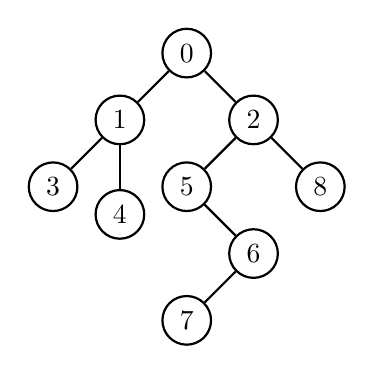
\begin{tikzpicture}[node distance={12mm}, thick, main/.style = {draw, circle}] 
            \node[main] (0) {$0$}; 
            \node[main] (1) [below left of=0] {$1$};
            \node[main] (2) [below right of=0] {$2$}; 
            \node[main] (3) [below left of=1] {$3$};            
            \node[main] (4) [below of=1] {$4$}; 
            \node[main] (5) [below left of=2] {$5$};            
            \node[main] (8) [below right of=2] {$8$}; 
            \node[main] (6) [below right of=5] {$6$}; 
            \node[main] (7) [below left of=6] {$7$};  
            \draw (0) -- (1); 
            \draw (0) -- (2); 
            \draw (1) -- (3);
            \draw (1) -- (4); 
            \draw (2) -- (5); 
            \draw (2) -- (8);
            \draw (5) -- (6); 
            \draw (6) -- (7); 
            \end{tikzpicture} 
        \end{center}
    \item Clearly, the longest path is $0\rightarrow 2 \rightarrow 5 \rightarrow 6 \rightarrow 7$
    \item Let the levels in the tree start from 1. For the induction step, we assume that the sub-problems at level 3 return the longest sub-problem. Now, we need to prove that nodes at level 2 will also return the optimal solution to its sub-problem.
    \item Lets consider the right part of the tree which consists of the actual longest path. At level 3, 'node 5' will return the array [7, 6, 5] and 'node 8' will return only [8] in their recursion respectively.
    \item Now, we need to prove that 'node 2' at level 1 will also return the optimal solution to its sub-problem. Length of array returned by 'node 5' is 3 and the one returned by 'node 8' is 1. We compare the lengths of the left and the right sub-problems, add the current node to the array with bigger size and return that array to its parent node. Consequently, 'node 2' will be added to the array returned by 'node 5', giving us [7, 6, 5, 2], which is clearly the optimal solution of the sub-problem at 'node 2'.    
    \item Thus, we conclude that if sub-problems at level i+1 in the tree return an optimal solution, the nodes at higher levels will always return the optimal solution as well. This proves the induction hypothesis.
    \item \textbf{Termination :} As we follow a bottom-up approach in solving the longest path problem from the root, the algorithm will always terminate once it reaches back to the root node and all the lower nodes are traversed once. 
\end{itemize}
\subsection{Analysis of Running Time}
\begin{itemize}
    \item We compute the runtime of this algorithm using the Master Theorem.
    
    \item The equation for Master Theorem is stated as follows:
    \begin{equation}
        T(n) = aT(n/b) + f(n) 
    \end{equation}
    where, 
        n = problem size \\
        a = number of subproblems in the recursion and a geq 1 \\
        n/b = size of each subproblem \\
        f(n) = cost of work done outside the recursive calls like dividing into subproblems and cost of combining them to get the solution. 
    \item As we are dealing with a binary tree, at every level of recursion the problem is reduced to 2 subproblems of at most n/2 size. Every recursion performs work for constant time c, so f(n) = O(1). Thus, substituting n = 2, n/b = n/2 and f(n) = 1 in equation (1).
    
    \begin{align*}
        T(n) &= 2T(n/2) + 1 && \text{level 1 recursion}\\
       T(n/2) &= (2^{2}T(n/2^{2}) + 1) + 1 && \text{level 2 recursion}\\
       &= 4T(n/4) + 2 \\
       T(n/4) &= 2^3(T(n/2^{3}) + 2) + 1 && \text{level 3 recursion}\\
       &= 8T(n/8) + 3
       .\\
       .\\
       .\\
       .
   \end{align*}
    From the above recursions, we  get, at level k,
       \begin{align*}
       T(n/2^{k-1}) &= 2^k\cdot T(n/2^k) + k && \text{(2)}\\ 
       \end{align*}
       When we reach the last subproblem, it means we have reached leaf node thus n/b = 1
       \begin{align*}
           n/2^k &= 1\\
           k &= log_2n\\
       \end{align*}
       Substituting this in equation (2)
       \begin{align*}
           T(n) &= 2^{log_2n}\cdot T(1) + log_2n && \text{(3)}\\ 
       \end{align*}
       As $2^{log_2n} = n^{log_22}$ and $log_22 = 1, T(1) = 1$
       \begin{align*}
           T(n) &= n + log_2n\\
           &= O(n)
       \end{align*}
    Thus, the asymptotic time complexity of the above algorithm is O(n).
\end{itemize}
\subsection{Longest Path of Weighted  Tree}
\begin{itemize}
    \item In order to find the longest path in a weighted binary tree, we just need to make a minor change in the recursion algorithm.
    \item Instead of adding nodes to the longest path list by comparing the length of left and right subtrees, we select the node to be added based on the weight of the subtrees. 
    \item The function getLongestPath() will return an Object of type LongestP{LP[], weight}, where LP[] is the array of nodes in the longestPath, while weight is the weight of the longestPath detected.
    \item Every node will have two additional parameters, weightLeft and weightRight. These weights will be added to the overall weight of the longestPath while traversing the tree branches.
    \item The recursive function getLongestPath(currentNode) can be modified to getLongestPathWeightTree(cuurentNode, weight) as follows to get the longest path in weighted binary trees. 
    
    \begin{algorithm}[H]
    \begin{algorithmic}
    
    \Function{getLongestPathWeightTree}{$currentNode, weight$}
    
    \If{$currentNode = null$}
        \State \Return emptyList
    \EndIf
    \State $rightW \gets currentNode.weightRight + weight$
    \State $leftW \gets currentNode.weightLeft + weight$
    \State $lpRight \gets getLongestPath(currentNode.right, rightW)$
    \State $lpLeft \gets getLongestPath(currentNode.left, leftW)$
    
    \If{$lpLeft.weight > lpRight.weight$}
        \State $lpLeft.LP \gets lpLeft.LP \cup currentNode.data$
        \State \Return lpLeft
    \Else
        \State $lpRight.LP \gets lpRight.LP \cup currentNode.data$
        \State \Return lpRight
    \EndIf
    
    \EndFunction
    \end{algorithmic}
    \end{algorithm}
    
    \item The recursion will be called as follows LongestP lp $\gets getLongestPathWeightTree(root, 0)$ 
    \item This algorithm will also take O(n) time to run, similar to the first algorithm.
\end{itemize}


\section{Problem 3 - Finding largest element in circularly shifted sorted array}
Suppose you are given an array A[1..n] of distinct sorted integers that have been circularly shifted
k positions to the right (for an unknown k). For example, [35, 42, 5, 15, 27, 29] is a sorted array that has been
circularly shifted k = 2 positions, while [27, 29, 35, 42, 5, 15] has been shifted k = 4 positions.
We can obviously find the largest element in A in O(n) time. Describe an O(log n) algorithm.
\subsection{Pseudocode}
We use a divide and conquer approach to find the largest element. The following recursive function (findMax) is used by the algorithm.
  \begin{algorithm}[H]
    \begin{algorithmic}
    
    \Function{findMax}{$A, left, right$}
    \If{$left = right$}
        \State \Return A[left]
    \EndIf
    \State $mid \gets (right + left)/ 2$  \Comment{If (right+left) is odd we floor mid}
    \If{$A[mid] > A[mid+1]$ }
        \State \Return A[mid]
    \ElsIf{$A[left] > A[mid]$}
        \State \Return findMax(A, left, mid-1)
    \Else
        \State \Return findMax(A, mid+1, right)
    \EndIf
    \EndFunction
    \end{algorithmic}
    \end{algorithm}
    
\begin{algorithm}[H]
    \caption{Find largest element in array}\label{alg:mst}
    \begin{algorithmic}
    \State $\textbf{Input : } $
    {\textbf{A - } Sorted array, circularly shifted right k times} 
    \State $size \gets$ size of array A
    \State \Return findMax(A, 0, size-1)
    \end{algorithmic}
\end{algorithm}
\subsection{Proof of Correctness}
\begin{itemize}
    \item To solve this problem, we take advantage of the fact that the array is sorted. If the array is not rotated at all (k=0), the largest element is the last element. 
    \item But, when the array is circularly shifted right k times, we notice that the only element with next element smaller than itself is the max element. 
    \item We take advantage of this observation to solve the problem in O(log n).
    \item At every iteration we reduce the search space by half, by selecting the portion of the array where the maximum element is. In order to identify the portion of array with the maximum element, we  analyze the left side. If the first element on the left side is larger than the mid element, it means that the max element is in this side. If not, it means the left part is properly sorted and max element is on the right side.
    \item We prove the algorithm using the method of induction. As we are using divide and conquer to solve this algorithm, the size of search space reduces by half every iteration. Thus, we use the problem size as the variable in our proof by induction. We try to prove that if our algorithm works for a problem size n, then it also works for size n+1.
    \item \textbf{Proof:}
    \begin{itemize}
        \item Let left be the index  of the first element and right be the index of the last element in the search array. Let mid = $\floor{(left + right)/2}$ be the index of the middle element. 
        \item Let n be the size of the problem such that n = right - left. Let x be the largest element in the array that we have to find.
        \item \textbf{Base Case : } The problem size = 1, that is n = 0 and right = left = mid. As the array has only one element, it will always be the largest one and we will always get the solution.
        \item \textbf{Induction : }We assume that we are able to find x in an array of size (right - left) $\leq$ n. We have to prove that our algorithm will work for a problem size of n+1 as well. We come across 3 cases as follows:
        \begin{itemize}
            \item  \textbf{Case 1 : $array[mid] > array[mid+1]$} \\
            As the array is sorted and rotated, it is obvious that x is the only element whose next element is smaller than itself. So, if the above condition is met, we have found a solution.
            \item \textbf{Case 2 : $array[left] > array[mid]$} \\
            The left portion must be in increasing order of elements for a sorted array. But, the first element being larger than the middle element indicates that x was shifted to the left of the middle element by circular rotation and must be present in this part. So, we explore only this part of the array by reducing the problem size to $\floor{(right-left)/2}$-1- left $leq$ n. According to the assumption made in the induction step, we are able to find the solution to problem sizes $\leq$ n.
            \item \textbf{Case 3 :} \\
            If the above two cases are not met, it means that x is present to the right of the middle element in the array. Thus, we have to explore only that part of the array and we reduce the problem size as $right-\floor{(right-left)/2}+1 \leq n$. As we can find the solution in search space of this size, according to the induction hypothesis, our algorithm is correct.
        \end{itemize}
        \item \textbf{Termination : } The algorithm will run recursively until it meets either of the termination conditions. If the search space left is of size 1, or if the next element is lesser than the current mid element. As a solution is found for every case in the induction step, the algorithm will always terminate. 
    \end{itemize}
\end{itemize}
\subsection{Analysis of Running Time}
\begin{itemize}
    \item The algorithm we used is a divide and conquer approach, where constant work c is performed in every recursion. If the solution is not found in that recursion, the problem is further reduced to a size of at most n/2. Thus, the recursion will end when n=2.
    \item Let T(n) represent the running time of the algorithm on input of size n.
    \begin{equation}
        T(n) \leq T(n/2) + c
    \end{equation}
    where, $n>2$ and $T(2) \leq c$
    \item We prove the running time of the algorithm by unrolling recursions. We do this in the following 3 steps:\\\\
        \textbf{Analyzing first few recursions }
        \begin{itemize}
        \item At the first recursion, the problem size is n. It runs in a constant time c.
        \item At level 2, the problem size is reduced to at most n/2 and it again runs for a constant time c.
        \item Level 3 has at most n/4 input size and it runs for another c time.
        \end{itemize}
        \textbf{Identify a pattern }
        \begin{itemize}
            \item From the above recursions, we derive that at every level j, the problem size is reduced to at most $n/2^{j}$ and every recursion contributes c to the overall running time.
        \end{itemize}
        \textbf{Summing runtime of all recursions}
        \begin{itemize}
            \item There are a total of $log_2n$ levels of recursion  till n reaches 2.
            \item Each recursion contributes a constant c to the runtime irrespective of its level j.
            \item Thus the total time complexity is denoted by $clog_2n$ = O(log n)
        \end{itemize}

\end{itemize}

\section{References}
\begin{enumerate}
    \item https://www.cs.cornell.edu/courses/cs211/2006sp/Lectures/L06-Induction/binary\_search.html
    \item https://www.geeksforgeeks.org/advanced-master-theorem-for-divide-and-conquer-recurrences/ 
    \item Lecture Notes by Prof. Alin Dobra
    \item Algorithm Design - Jon Kleinberg, Eva Tardos
    \item https://graal.ens-lyon.fr/~abenoit/algo09/coins2.pdf
\end{enumerate}
\end{document}
\documentclass[12pt]{article}

